% ======================================================
%  4 — SURPRISAL
% ======================================================
\section{Surprisal-Based Difficulty Modeling}

% --- 4.1 What is surprisal ---
\begin{frame}{What Is Surprisal?}
  \begin{columns}[c]
    \column{0.55\textwidth}
      \small
      From \textbf{information theory}:\\[0.5em]
      \begin{equation*}
        \text{Surprisal}(w_i) = -\log_2 P(w_i \mid w_1, \ldots, w_{i-1})
      \end{equation*}
      \vspace{0.8em}
      \textbf{Intuition:}\\[0.3em]
      \begin{itemize}
        \setlength\itemsep{0.5em}
        \item High surprisal $\rightarrow$ unexpected word $\rightarrow$ \textbf{harder}
        \item Low surprisal $\rightarrow$ predictable word $\rightarrow$ \textbf{easier}
      \end{itemize}
    \column{0.45\textwidth}
      \centering
      \begin{tikzpicture}
        \draw[->, thick] (0, 0) -- (5, 0) node[right, font=\scriptsize] {$P(w)$};
        \draw[->, thick] (0, 0) -- (0, 4) node[above, font=\scriptsize] {Surprisal};
        \draw[unisired, line width=2pt, domain=0.15:4.5, samples=100]
          plot (\x, {-1.2*ln(\x/5)});
        \fill[unisired] (0.5, 2.9) circle (3pt);
        \node[font=\scriptsize, right] at (0.7, 3.15) {\textbf{Hard clue}};
        \fill[unisired!40] (3.5, 0.45) circle (3pt);
        \node[font=\scriptsize, right] at (3.7, 0.7) {Easy clue};
      \end{tikzpicture}
  \end{columns}
\end{frame}

% --- 4.2 Key question ---
\begin{frame}{The Research Question}
  \begin{center}
    \vspace{1em}
    {\Large Can an LLM's \textbf{surprisal} predict\\[0.4em]
    how \textbf{difficult} a crossword clue is \textbf{for humans}?}
    \vspace{2em}

    \begin{tikzpicture}[
      box/.style={draw=unisired, rounded corners=8pt, minimum width=3.5cm, minimum height=1.3cm, align=center, font=\small, line width=1pt},
      arr/.style={->, >=Stealth, line width=1.5pt, unisired!50}
    ]
    \node[box, fill=unisired!8] (clue) at (0, 0) {Crossword\\Clue};
    \node[box, fill=unisired!8] (llm) at (5.5, 0) {LLM computes\\Surprisal};
    \node[box, fill=unisired!8] (diff) at (11, 0) {Predicted\\Difficulty};
    \draw[arr] (clue) -- (llm);
    \draw[arr] (llm) -- (diff);
    \end{tikzpicture}

    \vspace{1.5em}
    {\small\color{graytext} If yes $\Rightarrow$ we can \textbf{automatically calibrate} puzzle difficulty\\
    to match the learner's level --- no human annotation needed.}
  \end{center}
\end{frame}

% --- 4.3 Results ---
\begin{frame}{Surprisal Correlates with Human Performance}
  \begin{columns}[c]
    \column{0.5\textwidth}
      \centering
      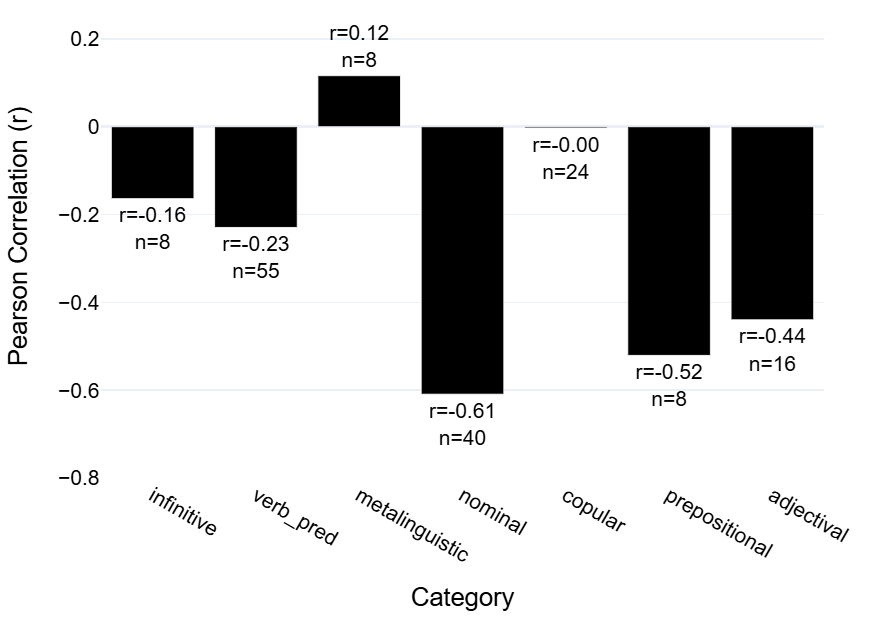
\includegraphics[width=\textwidth]{figures/accuracy-surprisal-macroGPT2.png}
    \column{0.5\textwidth}
      \begin{center}
        {\fontsize{38}{46}\selectfont\color{unisired}\textbf{$r \approx -0.57$}}\\[0.5em]
        {\large correlation with\\human accuracy}\\[1.5em]
        {\small Higher surprisal\\$\Rightarrow$ lower human accuracy}\\[1em]
        {\small\color{graytext} Effect is \textbf{stronger for nominal clues}\\
        (definition-style --- the most common type)}
      \end{center}
  \end{columns}
\end{frame}

% --- 4.4 Implications ---
\begin{frame}{Adaptive Difficulty for Education}
  \begin{center}
    \vspace{0.5em}
    \begin{tikzpicture}[
      level/.style={draw=unisired!40, rounded corners=8pt, minimum width=10.5cm, minimum height=1.2cm, align=center, font=\small, line width=0.7pt},
    ]
    \node[level, fill=green!8] at (0, 2.5) {
      {\color{green!50!black}\textbf{Easy}} --- Low surprisal clues $\rightarrow$ Beginners / Primary school
    };
    \node[level, fill=yellow!12] at (0, 0.8) {
      {\color{yellow!40!black}\textbf{Medium}} --- Moderate surprisal $\rightarrow$ Secondary school
    };
    \node[level, fill=red!8] at (0, -0.9) {
      {\color{unisired}\textbf{Hard}} --- High surprisal clues $\rightarrow$ Advanced / Expert
    };
    \draw[->, >=Stealth, line width=2pt, unisired!35] (6.3, 2.8) -- (6.3, -1.2);
    \node[font=\small, text=graytext, rotate=-90] at (7, 0.8) {Increasing surprisal};
    \end{tikzpicture}

    \vspace{1.8em}
    {\large Surprisal enables \textbf{automatic difficulty calibration}\\[0.2em]
    without manual annotation.}
  \end{center}
\end{frame}